\documentclass[12pt,letterpaper]{article}
\usepackage[utf8]{inputenc}
\usepackage[spanish]{babel}
\usepackage{graphicx}
\usepackage[left=2cm,right=2cm,top=2cm,bottom=2cm]{geometry}
\usepackage{graphicx} % figuras
% \usepackage{subfigure} % subfiguras
\usepackage{float} % para usar [H]
\usepackage{amsmath}
%\usepackage{txfonts}
\usepackage{stackrel} 
\usepackage{multirow}
\usepackage{enumerate} % enumerados
\renewcommand{\labelitemi}{$-$}
\renewcommand{\labelitemii}{$\cdot$}
% \author{}
% \title{Caratula}
\begin{document}

% Fancy Header and Footer
% \usepackage{fancyhdr}
% \pagestyle{fancy}
% \cfoot{}
% \rfoot{\thepage}
%

% \usepackage[hidelinks]{hyperref} % CREA HYPERVINCULOS EN INDICE

% \author{}
\title{Caratula}

\begin{titlepage}
\begin{center}
\large{UNIVERSIDAD PRIVADA DE TACNA}\\
\vspace*{-0.025in}
\begin{figure}[htb]
\begin{center}

\includegraphics[width=8cm]{./Imagenes/logo}
\end{center}
\end{figure}
\vspace*{0.15in}
INGENIERIA DE SISTEMAS  \\

\vspace*{0.5in}
\begin{large}
TITULO:\\
\end{large}

\vspace*{0.1in}
\begin{Large}
\textbf{PRACTICA DE LABORATORIO N 03} \\
\textbf{Creando un Reporte Interactivo en Power BI} \\
\end{Large}

\vspace*{0.3in}
\begin{Large}
\textbf{CURSO:} \\
\end{Large}

\vspace*{0.1in}
\begin{large}
INTELIGENCIA DE NEGOCIOS\\
\end{large}

\vspace*{0.3in}
\begin{Large}
\textbf{DOCENTE(ING):} \\
\end{Large}

\vspace*{0.1in}
\begin{large}
 Patrick Cuadros Quiroga\\
\end{large}

\vspace*{0.2in}
\vspace*{0.1in}
\begin{large}
Integrante: \\
\begin{flushleft}
Mamani Limache, Jhony 		\hfill	(2013046566) 
\end{flushleft}
\end{large}
\end{center}

\end{titlepage}


\tableofcontents % INDICE
\thispagestyle{empty} % INDICE SIN NUMERO
\newpage
\setcounter{page}{1} % REINICIAR CONTADOR DE PAGINAS DESPUES DEL INDICE


\begin{center}
    PRACTICA DE LABORATORIO N° 02
\end{center}

\section{OBJETIVOS}
A.

\section{REQUERIMIENTOS}

\begin{itemize}

- Conocimientos básicos de administración de base de datos Microsoft   SQL Server.
\\- Conocimientos básicos de SQL.
\\- Microsoft SQL Server 2016 o superior
\\- Base de datos AdventureWorks2016 o superior
\\- Power BI Desktop.
\\- Tener una cuenta Microsoft registrada en el Portal de Power Bi.
\end{itemize}

\section{DESARROLLO} 

\begin{itemize}
    Ejercicio 1: Conectando a Power BI a datos \\\\
    Tarea 1: Conectar a datos existentes\\\\
    1.  Abrir SQL Server Management Studio, y conectar a la instancia de base de datos (local) utilizando
        autenticación de Windows\\
    2.  En el menú Archivo (File), en el submenu Abrir (Open), hacer click en Project/Solution, y buscar el       archivo Project.ssmssln.\\
    3.  En el Explorador de Soluciones, expandir Consultas (Queries), y luego hacer doble click en el archivo     Lab Exercise 1.sql\\
    4.  Abrir Power BI Desktop\\
    5.  En la ventana Power BI Desktop, hacer click en Obtener Data (Get Data)\\
    6.  En el cuadro Obtener Datos, click base de datos Microsoft SQL, y entonces click en Conectar\\
    7.  En la ventana base de datos Server database, En Servidor, escribir (local).\\
    8.  En Base de Datos (opcional), tipear AdventureWorksLT.\\
    9.  Expandir el cuadro Opciones Avanzadas. Copiar el script Task 1 del archivo Lab Exercise 1.sql. y       pegar la consulta en Power BI, en el cuadro sentencia SQL. Luego presionar OK.\\
    10.  En la ventana de vista preliminar click en Cargar.\\
    11.  En Power BI Desktop, click Obtener Datos y luego click en Mas\\
    12.  Repetir los pasos del 6 al 10, utilizando el script Task 2\\
    13.  De regreso en el reporte. Guardar el archivo como AdventureWorksLT Sales.pbix.\\

\end{itemize} 

\begin{center}
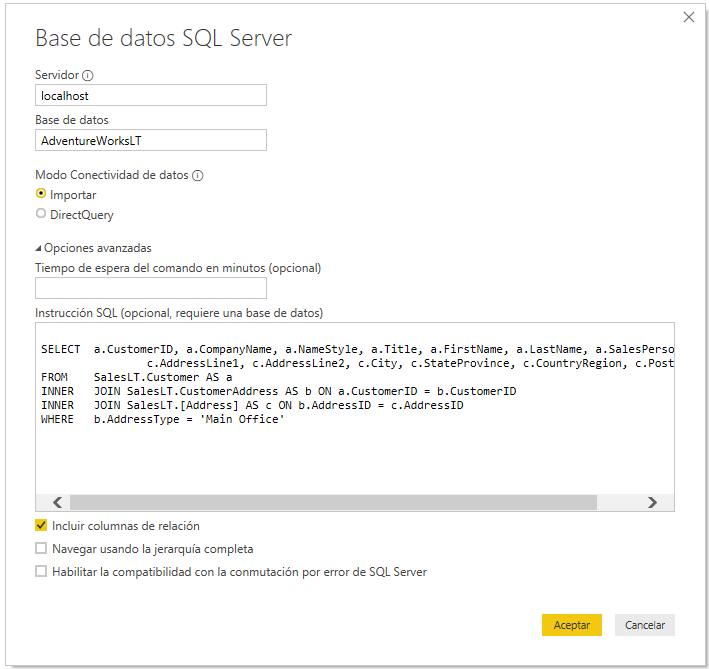
\includegraphics[width=12cm]{./Imagenes/img_01} 
\end{center}

\begin{center}
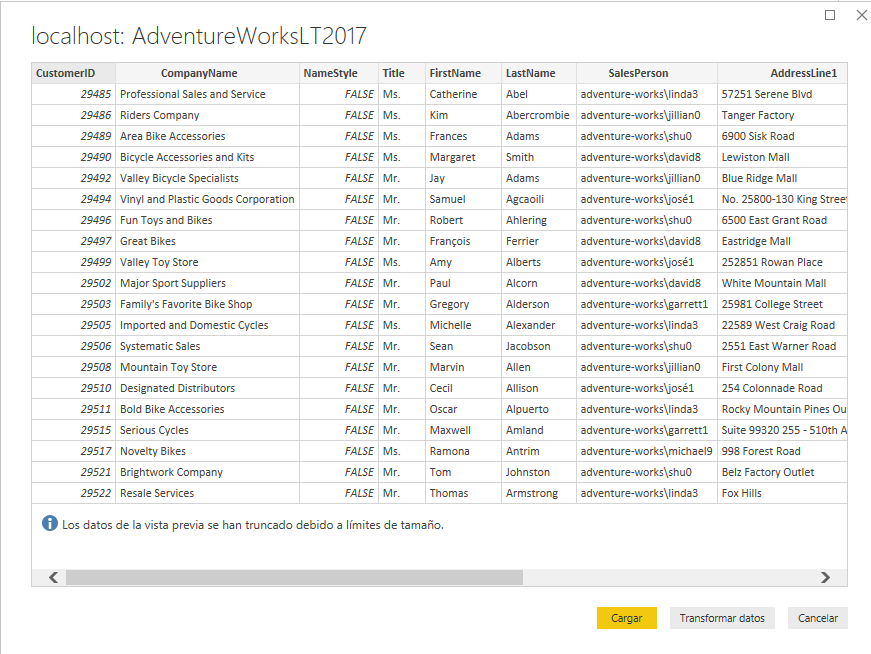
\includegraphics[width=12cm]{./Imagenes/img_02} 
\end{center}
    
\begin{center}
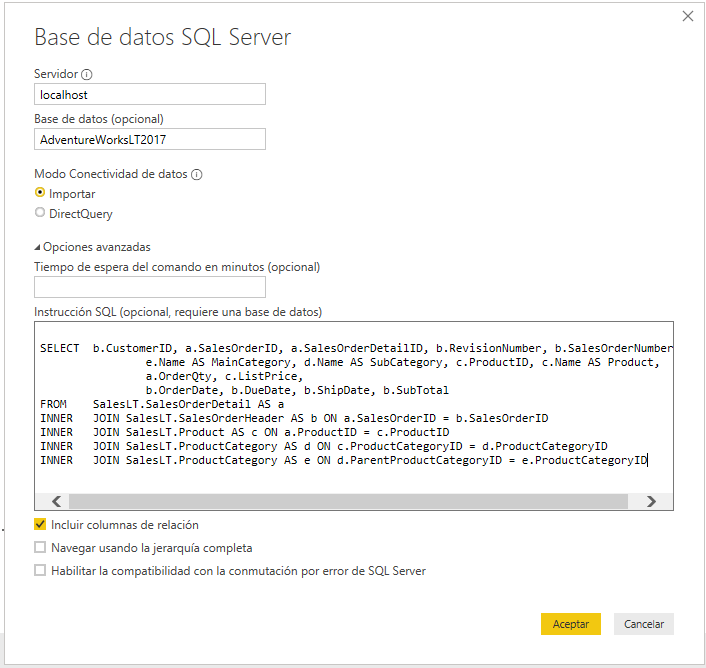
\includegraphics[width=12cm]{./Imagenes/img_03} 
\end{center}

\begin{center}
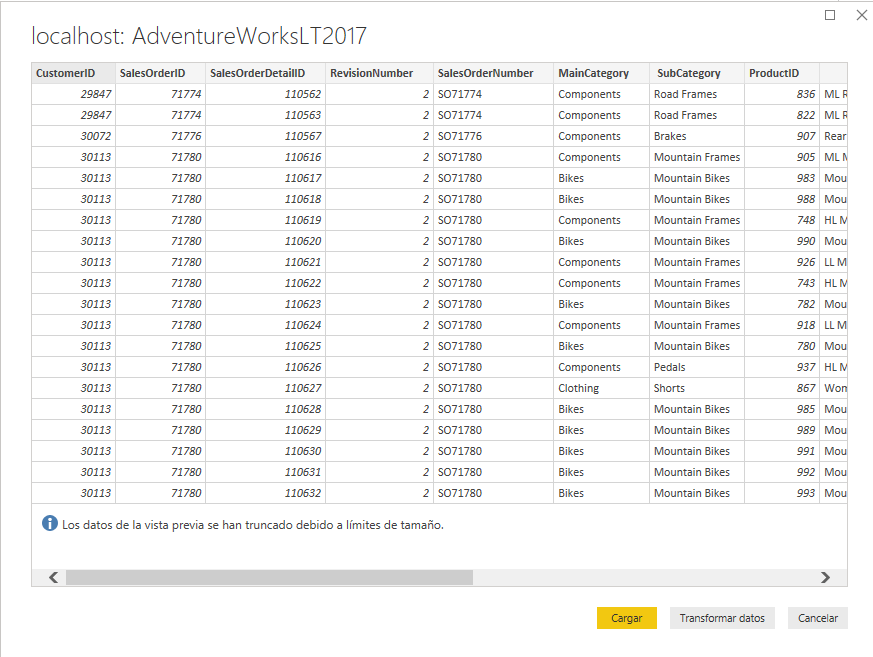
\includegraphics[width=12cm]{./Imagenes/img_04} 
\end{center}
    
    
\begin{itemize}
    
    Tarea 2: Graficar Datos\\\\
    1.  En el panel Campos (Fields), click derecho sobre Query1, Renombrar, tipear Customers y presionar Enter\\
    2.  En el menú Archivo (File), en el submenu Abrir (Open), hacer click en Project/Solution, y buscar el       archivo Project.ssmssln.\\
    3.  En el Explorador de Soluciones, expandir Consultas (Queries), y luego hacer doble click en el archivo     Lab Exercise 1.sql\\
    4.  Abrir Power BI Desktop\\
    5.  En la ventana Power BI Desktop, hacer click en Obtener Data (Get Data)\\
    6.  En el cuadro Obtener Datos, click base de datos Microsoft SQL, y entonces click en Conectar\\
    7.  En la ventana base de datos Server database, En Servidor, escribir (local).\\
    8.  En Base de Datos (opcional), tipear AdventureWorksLT.\\
    9.  Expandir el cuadro Opciones Avanzadas. Copiar el script Task 1 del archivo Lab Exercise 1.sql. y       pegar la consulta en Power BI, en el cuadro sentencia SQL. Luego presionar OK.\\
    10.  En la ventana de vista preliminar click en Cargar.\\
    11.  En Power BI Desktop, click Obtener Datos y luego click en Mas\\
    12.  Repetir los pasos del 6 al 10, utilizando el script Task 2\\
    13.  De regreso en el reporte. Guardar el archivo como AdventureWorksLT Sales.pbix.\\

\end{itemize} 
    
    
    
    
    
    
\include{Secciones/Actividad02}
\include{Secciones/Actividad03}
\include{Secciones/Actividad04}




\end{document}
